Dette afsnit indeholder en gennemgang af grafisk brugergrænseflade, design og implementering af 'Project List' viewet i Rambøll Tilsyn.

\subsubsection{Design}
På figur \ref{fig:ProjctListSekvens} ses sekvens diagrammet for 'Project List' viewet til Rambøll Tilsyn.
%\begin{figure}[H] % (alternativt [H])
%	\centering
%	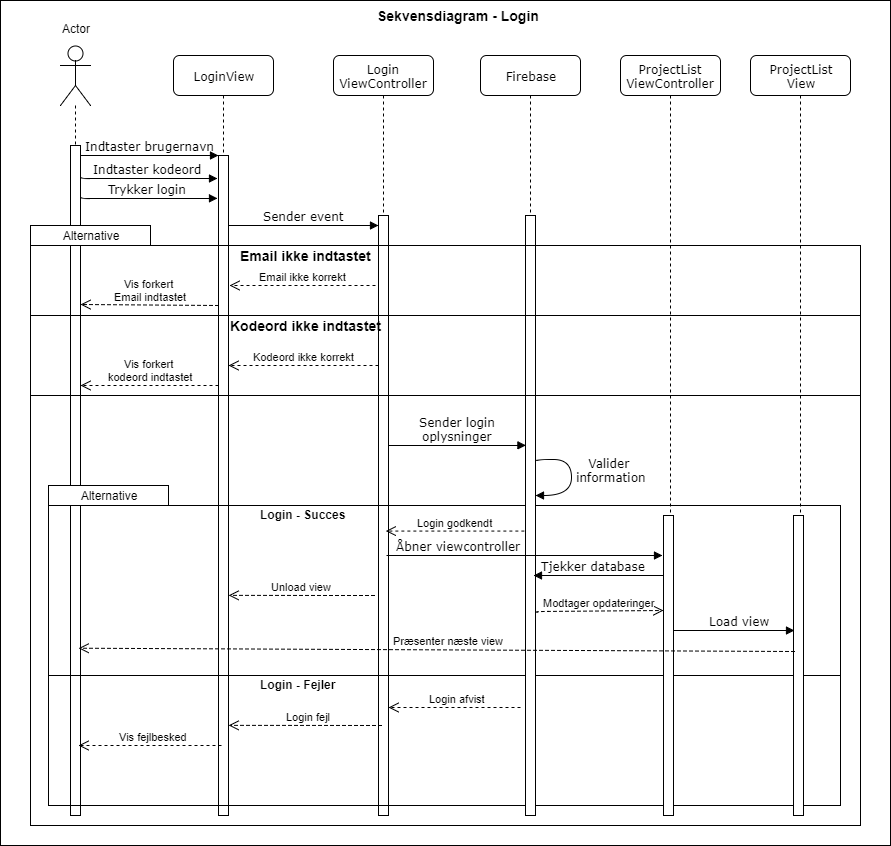
\includegraphics[height=15cm, width=15cm]{../ArkitekturDesign/Design/Login/LoginSekvensDiagram}
%	\caption{Sekvensdiagram for Login i Rambøll Tilsyn.}
%	\label{fig:ProjctListSekvens}
%\end{figure}

\clearpage

\subsubsection{Grafisk brugergrænseflade}
I LoginViewet er der lavet felter til at bruger indtaster sit brugernavn og kodeord. Se figur \ref{fig:ProjectListView}
\begin{figure}[H] % (alternativt [H])
	\centering
	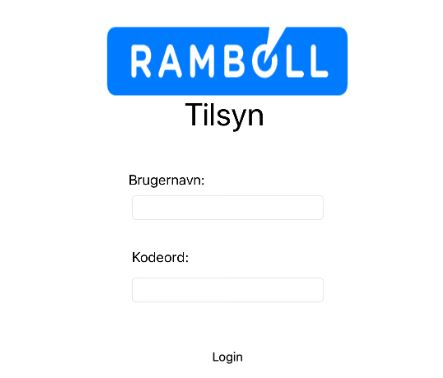
\includegraphics[height=12cm, width=10cm]{../ArkitekturDesign/Design/Login/LoginView}
	\caption{Login viewet som det er implementeret i Rambøll Tilsyn.}
	\label{fig:ProjectListView}
\end{figure}

\clearpage

\subsubsection{Implementering}
I dette afsnit vil der blive beskrevet funktionaliteten for de vigtigste funktioner i koden tilhørende 'Login' viewet.

På figur \ref{fig:Checkifusersigned}, ses funktionen for CheckIfUserSignedIn.
\begin{figure}[H] % (alternativt [H])
	\centering
	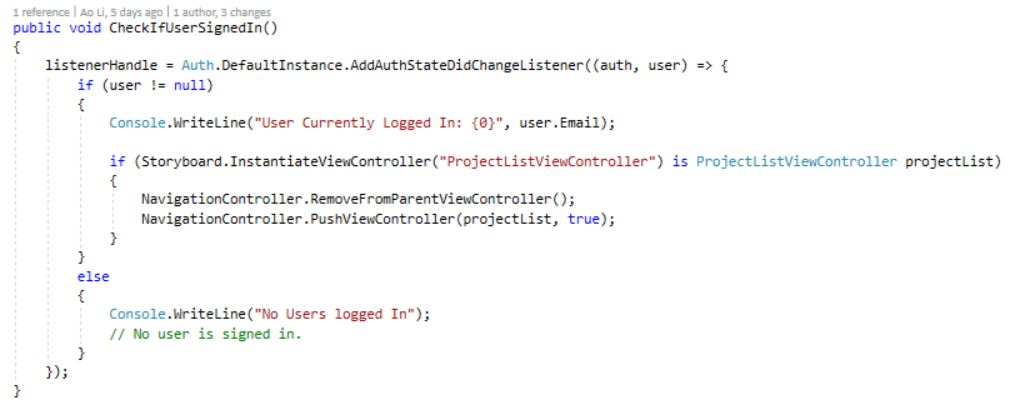
\includegraphics[height=8cm, width=15cm]{../ArkitekturDesign/Design/Login/Checkifusersigned}
	\caption{}
	\label{fig:Checkifusersigned}
\end{figure}
